\documentclass[14,fleqn]{article}
\usepackage{amsmath}
\usepackage{amssymb}
\usepackage[top=.5 in,left=.5 in,right=.5 in,bottom=.5 in]{geometry}
\usepackage{enumerate}
\usepackage{ mathrsfs }
\usepackage{graphicx}
\usepackage{pgf,tikz}
\usepackage{mathrsfs}
\usepackage{gensymb}
\usepackage{venndiagram}
\usetikzlibrary{arrows}

\pagenumbering{gobble}

\setlength{\parindent}{0 pt}
\setlength{\parskip}{1 ex}

\newcommand{\lcm}{\textnormal{lcm}}
\newcommand{\norm}{\triangleabove right}
\newcommand{\bfm}[1]{$\boldsymbol{#1}$}
\newcommand{\Z}{\ensuremath{\mathbb{Z}}}
\newcommand{\R}{\ensuremath{\mathbb{R}}}
\newcommand{\C}{\ensuremath{\mathbb{C}}}
\renewcommand{\wedge}[1]{\ensuremath{\langle #1 \rangle}}
\newcommand{\infsum}[1]{\ensuremath{\sum_{n=#1}^\infty}}
\newcommand{\defn}[1]{\textbf{\underline{#1}}}

%\begin{venndiagram3sets}[labelA=$S$,labelB=$T$,labelC=$U$]
%	\fillA
%	\fillOnlyC
%\end{venndiagram3sets}\\

%\begin{venndiagram2sets}[labelA=$S$,labelB=$T$]
%	\fillNotA
%	\fillNotB
%	\setpostvennhook{
%		\draw[] (labelAB) ++(0,-2.1) node {\raisebox{0pt}[0pt][0pt]{$(S\cap T)'$}};
%	}
%\end{venndiagram2sets}\\

\begin{document}
\section{Section 5.6: More Counting Principles}
In this section we want to apply the previous counting principles to more advanced situations where the solutions are not quite as obvious. But ideas like combinations can solve a variety of problems if we only view questions in the right way.

\textbf{Example:} Suppose we flip a coin 6 times in a row and record the outcomes. Answer the following questions.
\begin{enumerate}
	\item How many possible outcomes are there?
	\item How many outcomes start with a head?
	\item How many outcomes have exactly 2 tails?
	\item How many outcomes have at most 2 heads?
	\item How many outcomes have at most 3 tails?
	\item How many outcomes have at least 1 head?
\end{enumerate}

Answers:
\begin{enumerate}
	\item Multiplication principle gives $2^6=64.$
	\item Same as before but only one choice for the first flip so $1\cdot 2^5=32.$
	\item If a flip has exactly 2 tails the only thing to be determined is when the tails happened. There are 6 possible positions and we have to choose 2 of them. The order doesn't matter since tails are the same. If we choose 2 items from 6 without order this is a combination so there are $\binom{6}{2}=16$ possible outcomes.
	\item At most 2 heads means either 0,1, or 2 heads. So we use the same argument as before and add (since they are clearly disjoint) so we get $\binom{6}{0}+\binom{6}{1}+\binom{6}{2}=1+6+16=23.$
	\item At most 3 tails can be found the same was as the previous problem and we get $\binom{6}{0}+\binom{6}{1}+\binom{6}{2}+\binom{6}{3}=32.$ Alternatively, there must be the same number of at most 3 heads and at most 3 tails since there is no difference between heads and tails, and these choices cover all possibilites.
	\item At least 1 head should be the complement of no heads. So we can do $64-\binom{6}{0}=63.$ Use the complement rule $n(A')=n(U)-n(A).$
\end{enumerate}

Question for pondering. How many outcomes have exactly 1 head? How many outcomes have exactly 5 tails? How are these two related?

Next we consider some problems about grid paths. Consider the following grid representing a group of city blocks.
\begin{center}
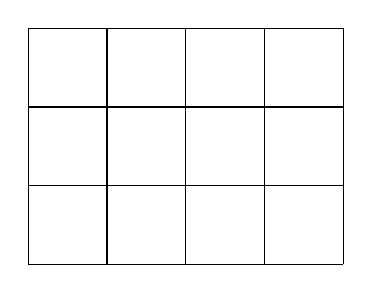
\begin{tikzpicture}
	\draw[step=1.0,black,thin] (0,0) grid (4,3);
\end{tikzpicture}
\end{center}
How many shortest paths are there fromt the bottom left to the top right corner? Examples include
\begin{center}
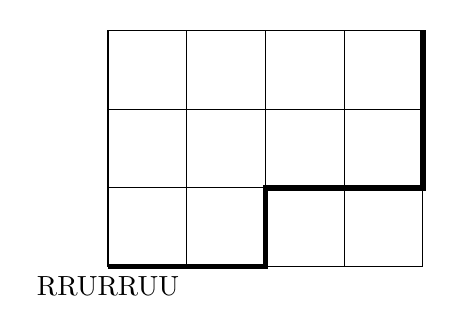
\begin{tikzpicture}
	\draw[step=1.0,black,thin] (0,0) grid (4,3);
	\draw[line width=2 pt] (0,0)--(2,0)--(2,1)--(4,1)--(4,3);
	\draw (0,0) node[below] {RRURRUU};
\end{tikzpicture}
\hfill
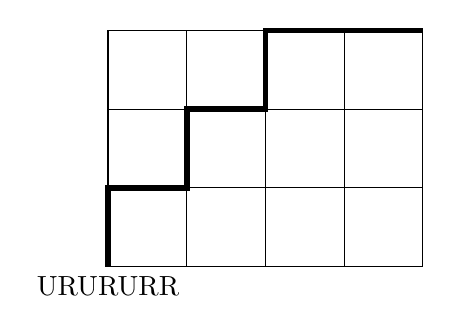
\begin{tikzpicture}
	\draw[step=1.0,black,thin] (0,0) grid (4,3);
	\draw[line width=2 pt] (0,0)--(0,1)--(1,1)--(1,2)--(2,2)--(2,3)--(4,3);
	\draw (0,0) node[below] {URURURR};
\end{tikzpicture}
\hfill
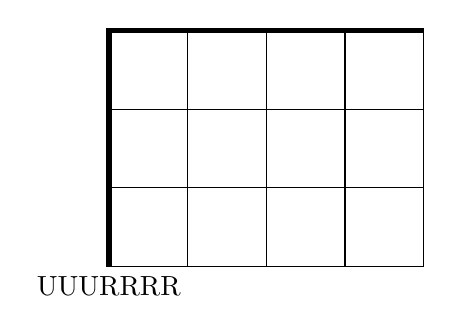
\begin{tikzpicture}
	\draw[step=1.0,black,thin] (0,0) grid (4,3);
	\draw[line width=2 pt] (0,0)--(0,3)--(4,3);
	\draw (0,0) node[below] {UUURRRR};
\end{tikzpicture}

\end{center}

How many block lengths do we have to travel to get from one corner to the other? How many of them are ``go right''? How many of them are ``go up''? For each path, make the following string: every time you go up, make a U and every time you go right, make an R. (Sequences are below the pictures.)

How many of these sequences are there? Does each sequence give a different path. This means that there are $\binom{7}{4}$ paths from the bottom left corner to the top right corner.

What if the grid was 7 squares tall and 3 squares wide? Can you use the same arguments as before? Determine how many shortest paths through the grid there are.

Two variations: Consider the following 5x3 grid\\
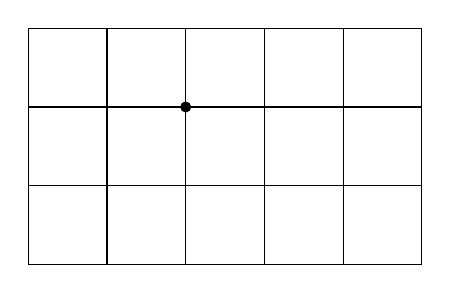
\begin{tikzpicture}
	\draw[step=1.0, black, thin] (0,0) grid (5,3);
	\fill (2,2) circle[radius=2 pt];
\end{tikzpicture}\\
How many shortest paths go through the dot? (Do a shortest path before the dot, then a shortest path after and multiply.)\\

How many shortest paths have the property that you never go up twice in a row?\\
This one is a little trickier. We could try and compute directly but that gets complicated. Instead lets put all rights down first, with spaces in between so we get \_R\_R\_R\_R\_R\_. Since we can't place any U's together, we can place at most 1 U in each blank. This means we just have to choose which blanks the U's go in. There are 6 blanks and 3 U's so there are $\binom{6}{3}$ different paths.\\
What if we wanted a path where we never go right twice in a row? How many of these are there?

Card Problems: We consider a standard 52 card deck with 4 suits and 13 cards in each suit. \textbf{Very Important:} The point of these questions is not the exact problem, but the techniques we use. It is difficult to teach exact problems because you can really only get better through practice and seeing a lot of different problem types.\\

For these problems we will will be drawing a standard 5 card poker hand. We will also assume that if we are looking for a given hand we don't have one better.
\begin{enumerate}
	\item How many different hands are there?
	\item How many different hands have 2 hearts and 3 clubs?
	\item How many different hands have at least one of each suit?
	\item How many hands have exactly 3 suits?
	\item How many different full houses are there?
	\item How many different flushes are there?
	\item How many 3 of a kind are there?
\end{enumerate}

Solutions:
\begin{enumerate}
	\item To make a poker hand we have to choose 5 of the 52 cards so there are $\binom{52}{5}$ possible hands.
	\item If a hand has 2 hearts and 3 clubs then we can choose one then the other. First we choose the two hearts. There are $\binom{13}{2}$ ways to do this. Then we choose the 3 clubs and there are $\binom{13}{3}$ ways to do this. Since we do these one after another we use the multiplication principle and get $\binom{13}{2}\binom{13}{3}.$
	\item If the hand has each suit then there will be one suit with exactly 2 cards. First we choose that suit and there are 4 ways to do this. Then we pick the two cards in that suit. Then we pick the 1 card in the other 3 suits. This gives $4\binom{13}{2}\cdot 13\cdot 13\cdot 13$
	\item Since there are 3 suits then there are two possibilites. Either two suits have 2 cards or 1 suit has 3 cards. These are disjoint sowe can find the number for each and add them together. First we consider the suit with 3 cards. Let's pick the 3 suits represented. Then from thse 3 we want to pick which one has 3 cards. Then for that suit we choose the 3 cards and then for the other two suits we pick 1 card. If two suits have 2 cards then we still pick the 3 suits, then pick which two suits have 2 cards. Then we pick the cards for each. Thus we get
		\[
			\binom{4}{3}\binom{3}{1}\binom{13}{3}\binom{13}{1}\binom{13}{1}+\binom{4}{3}\binom{3}{2}\binom{13}{2}\binom{13}{2}\binom{13}{1}
		\]
	\item A full house is three of the same care with 2 of the same card. Let's first choose the two card types, but in order so the first one has the 3 of a kind. So there are $P(13,2)$ ways to do this. Then for the first card type we need to choose 3 suits. Then for the second card type we choose 2 suits. So there are $P(13,2)\cdot \binom{4}{3}\binom{4}{2}$ full houses.
	\item A flush consists of a suit and 5 cards from that suit. So there are $4\cdot \binom{13}{5}$ ways to do this. But we should eliminate all of the straight flushes because those are a different hand. We can directly count there are $4\cdot 10$ of these so we subtract from before.
	\item For a 3 of a kind we need 3 different card types. Then we choose one of these to be the 3 of a kind, then we choose the cards for each. This gives $\binom{13}{3}\binom{3}{1}\binom{4}{3}\binom{4}{1}\binom{4}{1}.$
\end{enumerate}

So far we have mostly worked with indistinguishable objects. But what happens if they are different?\\
How many ways can 4 men and 5 women be arranged in a row so that no to men are next to each other?\\
First we choose how the men and women are placed. Using the same argument as before there are $\binom{6}{4}$ ways to do  this. Then we order the men and women separately so we get $\binom{6}{4} 5!4!$.


How many ways can 5 people be lined up so the tallest is to the left of the shortest?\\
Pick the places for the tallest and shortest. Their order is determined. Then order the other 3 however you want.\\
\end{document}
